\documentclass[12pt]{article}
\usepackage[a4paper, margin=0.75in]{geometry}
\usepackage[document]{ragged2e}
\usepackage{graphicx}
\graphicspath{ {./images/} }
\usepackage{enumerate}
\usepackage{framed}
\usepackage{amsmath,amsfonts,amsthm,thmtools,amssymb,mathtools,commath}
\usepackage{physics}
\usepackage{tikz}
\usetikzlibrary{mindmap}
\usepackage{caption}
\usepackage{xcolor}
\usepackage[most]{tcolorbox}
\usepackage{cleveref}


%%%%%%%%%%%%%%%%
%  Definition  %
%%%%%%%%%%%%%%%%
\tcbuselibrary{theorems,skins,hooks}
\newtcbtheorem[number within=subsection]{definition}{Definition}%
{
    % theorem style=definition,
    enhanced,
	before skip=2mm,after skip=2mm, colback=cyan!5,colframe=cyan!80!black,boxrule=0.5mm,
	attach boxed title to top left={xshift=1cm,yshift*=1mm-\tcboxedtitleheight},
	boxed title style={frame code={
					\path[fill=cyan]
					([yshift=-1mm,xshift=-1mm]frame.north west)
					arc[start angle=0,end angle=180,radius=1mm]
					([yshift=-1mm,xshift=1mm]frame.north east)
					arc[start angle=180,end angle=0,radius=1mm];
					\path[left color=cyan!30!black,right color=cyan!30!black,
						middle color=cyan!50!black]
					([xshift=-2mm]frame.north west) -- ([xshift=2mm]frame.north east)
					[rounded corners=1mm]-- ([xshift=1mm,yshift=-1mm]frame.north east)
					-- (frame.south east) -- (frame.south west)
					-- ([xshift=-1mm,yshift=-1mm]frame.north west)
					[sharp corners]-- cycle;
				},interior engine=empty,
		},
	fonttitle=\bfseries,
	title={#2},#1
}{def}


%%%%%%%%%%%%%
%  Theorem  %
%%%%%%%%%%%%%
\tcbuselibrary{theorems,skins,hooks}
\newtcbtheorem[use counter from=definition]{theorem}{Theorem}%
{
    theorem style=plain,
    enhanced,
    colframe=green,
    boxrule=1pt,
    titlerule=0mm,
    toptitle=1mm,
    bottomtitle=1mm,
    fonttitle=\bfseries,
    fontupper=\mdseries\itshape,
    coltitle=green!30!black,
    colbacktitle=cyan!15!white,
    colback=green!10,
    description font=\bfseries\sffamily
}{thrm}


%%%%%%%%%%%%%%
% Corollary  %
%%%%%%%%%%%%%%
 \tcbuselibrary{theorems,skins}
 \newtcbtheorem[use counter from=theorem]{corollary}{Corollary}%
 {
    theorem style=plain,
    enhanced,
    colframe=green,
    frame hidden,
    titlerule=0mm,
    toptitle=1mm,
    bottomtitle=1mm,
    fonttitle=\bfseries,
    fontupper=\mdseries\itshape,
    coltitle=green!30!black,
    colbacktitle=cyan!15!white,
    colback=green!10,
    description font=\bfseries\sffamily
 }{corl}


%%%%%%%%%%%%%
%  Example  %
%%%%%%%%%%%%%
\tcbuselibrary{theorems,skins,hooks}
\newtcbtheorem[number within=section]{example}{Example}%
{
	enhanced,
	breakable,
	colback = gray!5,
	frame hidden,
	boxrule = 0sp,
	borderline west = {2pt}{0pt}{gray},
	sharp corners,
	detach title,
	before upper = \tcbtitle\par\smallskip,
    coltitle=gray!70!black,
	fonttitle = \bfseries\sffamily,
	description font = \mdseries\bfseries
}
{xmp}


%%%%%%%%%%%%%%
%  Exercise  %
%%%%%%%%%%%%%%
\tcbuselibrary{theorems,skins,hooks}
\newtcbtheorem[number within=section]{exercise}{Exercise}%
{
    enhanced,
    breakable,
    colback=black!5,
    colframe=black!30,
    left=0.5em,
    before skip=10pt,
    after skip=10pt,
    boxrule=0pt,
    boxsep=0pt,
    arc=0pt,
    outer arc=0pt,
    borderline west={3pt}{0pt}{black!30},
}{exc}

%%%%%%%%%%
%  Note  %
%%%%%%%%%%
\usetikzlibrary{arrows,calc,shadows.blur}
\tcbuselibrary{skins}
\newtcolorbox{note}[1][]{%
	enhanced jigsaw,
	colback=gray!20!white,%
	colframe=gray!80!black,
	size=small,
	boxrule=1pt,
	title=\textbf{Note:-},
	halign title=flush center,
	coltitle=black,
	breakable,
	drop shadow=black!50!white,
	attach boxed title to top left={xshift=1cm,yshift=-\tcboxedtitleheight/2,yshifttext=-\tcboxedtitleheight/2},
	minipage boxed title=1.5cm,
	boxed title style={%
			colback=white,
			size=fbox,
			boxrule=1pt,
			boxsep=2pt,
			underlay={%
					\coordinate (dotA) at ($(interior.west) + (-0.5pt,0)$);
					\coordinate (dotB) at ($(interior.east) + (0.5pt,0)$);
					\begin{scope}
						\clip (interior.north west) rectangle ([xshift=3ex]interior.east);
						\filldraw [white, blur shadow={shadow opacity=60, shadow yshift=-.75ex}, rounded corners=2pt] (interior.north west) rectangle (interior.south east);
					\end{scope}
					\begin{scope}[gray!80!black]
						\fill (dotA) circle (2pt);
						\fill (dotB) circle (2pt);
					\end{scope}
				},
		},
	#1,
}


\title{
    \textbf{Experiment 7} \\
    \textbf{\Large Analyzing the frequency response of a single tuned amplifier to investigate the low pass frequency and high pass frequency.}
}

\author{
    Turja Roy \\
    ID: 2108052
}
\date{}

\begin{document}
\maketitle

\section{Objective}

\begin{enumerate}
    \item To draw and analyze the frequency response of a single tuned amplifier.
    \item To investigate the low pass frequency and high pass frequency by analyzing the frequency response graphs. 
    \item Establish a comprehensive understanding of the correlation between simulation and experimental data for the frequency response of a single tuned amplifier.
\end{enumerate}

\section{Circuit Diagram}

\begin{figure}[h!]
    \centering
    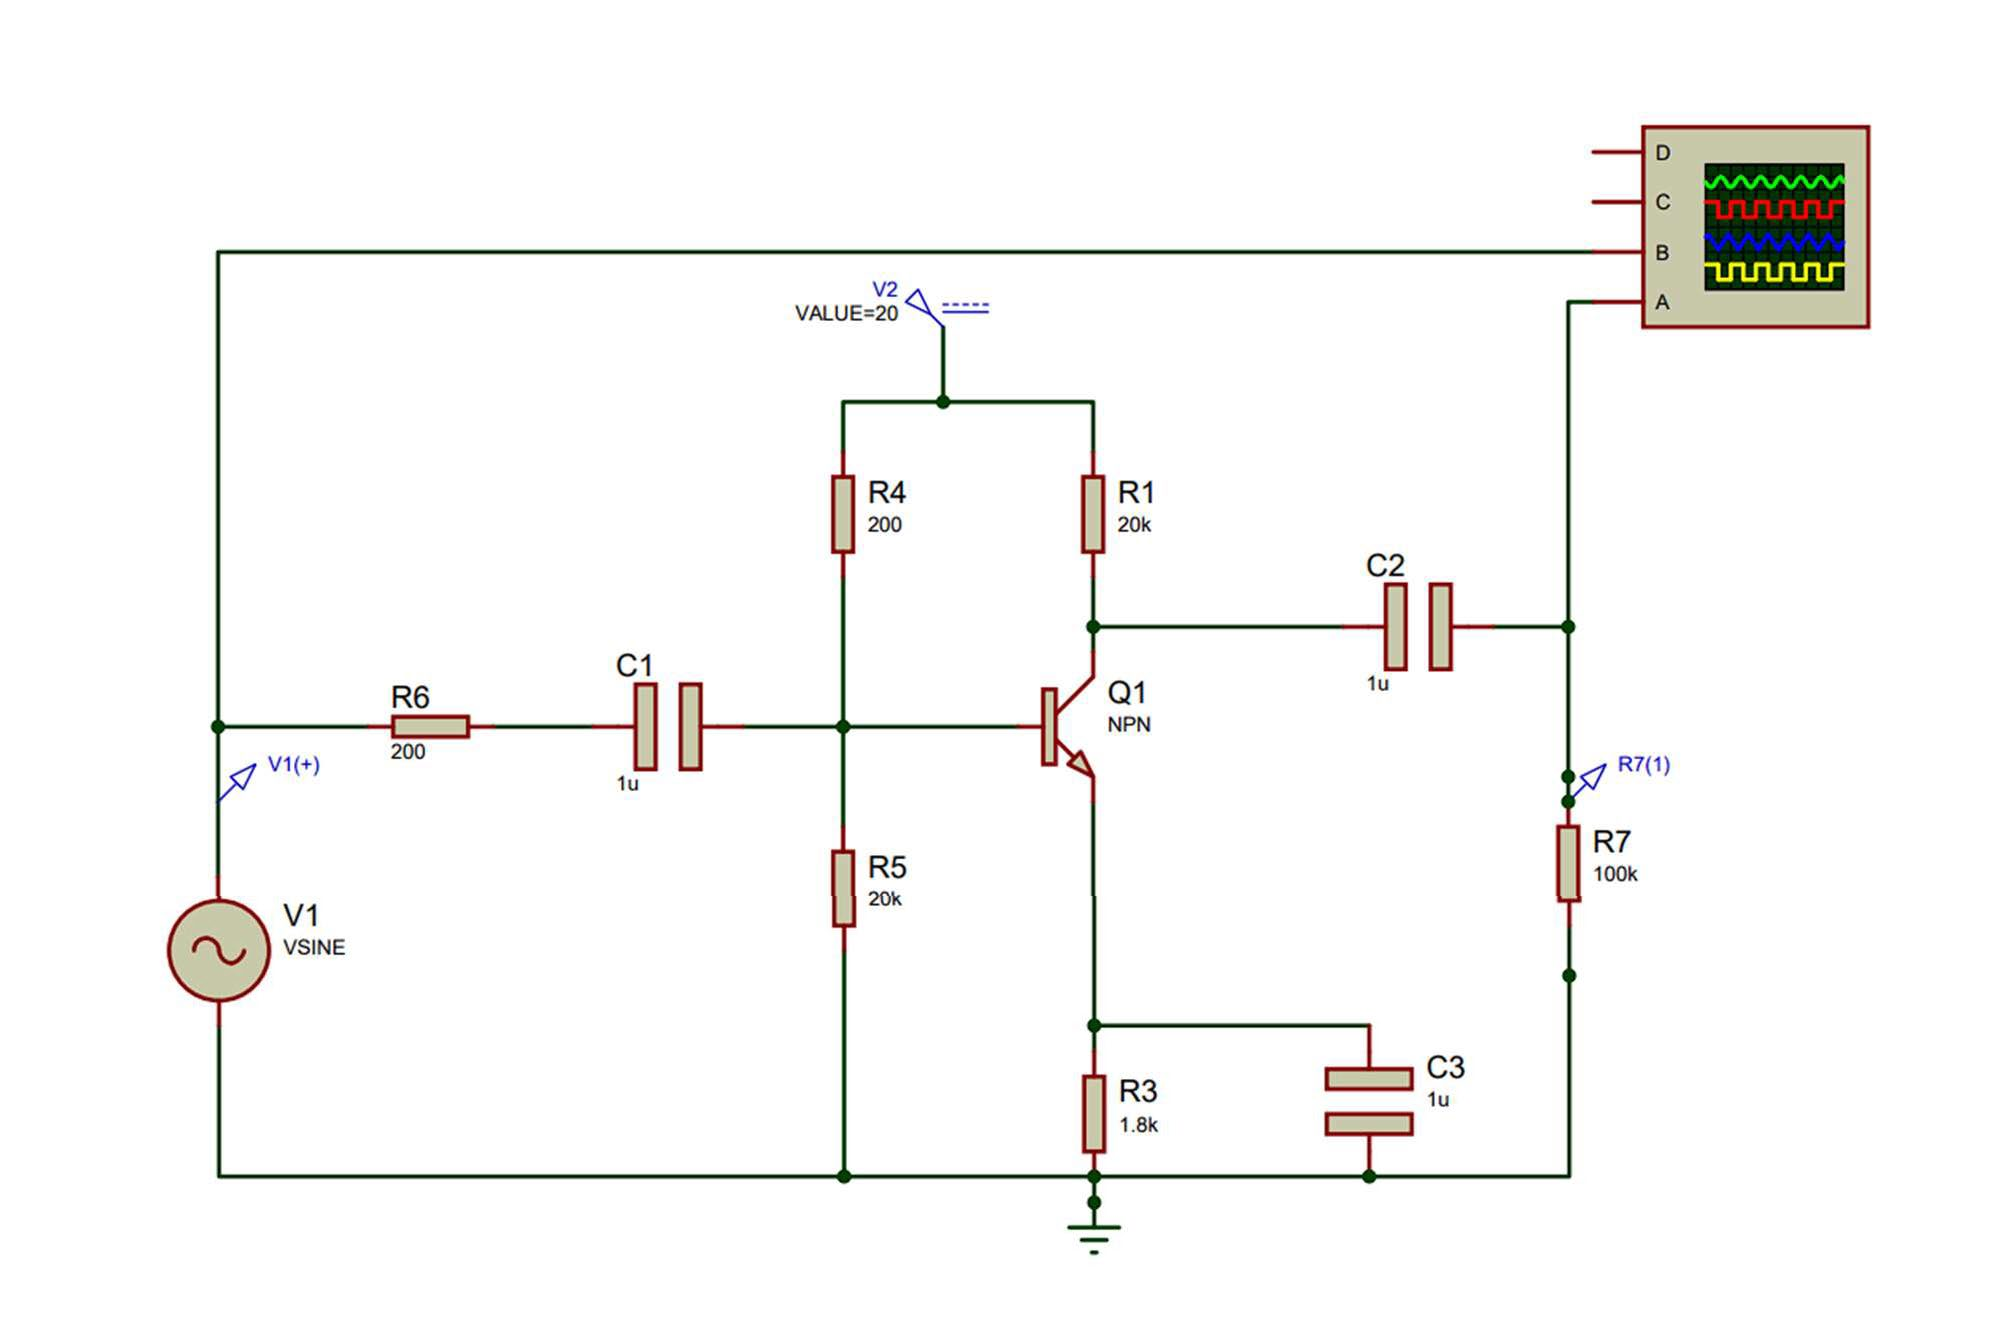
\includegraphics[width=.7\textwidth]{Circuit.png}
    \caption{Circuit Diagram for Determining Frequency Response.png}
\end{figure}

A voltage divider bias circuit was constructed using an NPN transistor and four resistors. The circuit included a bypass capacitor, C2. A DC voltage source was connected to the collector of the transistor. The input voltage,V1, was applied, and the output voltage was obtained from the load Resistor, R7. Figure 1 represents the circuit diagram.

\section{Result Analysis}

\subsection{Data Table}

\begin{table}[h!]
    \centering
    \caption{Experimental Data}
    \begin{tabular}{rrrrrr}
        \hline
        Vin (mV) &  Frequency &  Logarithmic Frequency &  Vout (mV) &  Av &  Gain (dB) \\
        \hline
        100 &         50 &                1.69897 &       2600 &  26 &  28.299467 \\
        100 &        100 &                2.00000 &       5000 &  50 &  33.979400 \\
        100 &        200 &                2.30103 &       9100 &  91 &  39.180828 \\
        100 &        500 &                2.69897 &      15000 & 150 &  43.521825 \\
        100 &       1000 &                3.00000 &      17000 & 170 &  44.608978 \\
        100 &       2000 &                3.30103 &      17800 & 178 &  45.008400 \\
        100 &       5000 &                3.69897 &      18000 & 180 &  45.105450 \\
        100 &      10000 &                4.00000 &      18000 & 180 &  45.105450 \\
        100 &      20000 &                4.30103 &      18000 & 180 &  45.105450 \\
        100 &      50000 &                4.69897 &      18000 & 180 &  45.105450 \\
        100 &     100000 &                5.00000 &      18000 & 180 &  45.105450 \\
        100 &     200000 &                5.30103 &      18000 & 180 &  45.105450 \\
        100 &     500000 &                5.69897 &      18000 & 180 &  45.105450 \\
        100 &    1000000 &                6.00000 &      18000 & 180 &  45.105450 \\
        100 &    2000000 &                6.30103 &      18000 & 180 &  45.105450 \\
        100 &    5000000 &                6.69897 &      16000 & 160 &  44.082400 \\
        100 &   10000000 &                7.00000 &      12000 & 120 &  41.583625 \\
        100 &   20000000 &                7.30103 &       7500 &  75 &  37.501225 \\
        100 &   40000000 &                7.60206 &       4000 &  40 &  32.041200 \\
        \hline
    \end{tabular}
\end{table}

\begin{table}[h!]
    \centering
    \caption{Simulation Data}
    \begin{tabular}{rrrrrr}
        \hline
        Vin (mV) &  Frequency &  Logarithmic Frequency &  Vout (mV) &    Av &  Gain (dB) \\
        \hline
        100 &         50 &                1.69897 &        380 &   3.8 &  11.595672 \\
        100 &        100 &                2.00000 &        600 &   6.0 &  15.563025 \\
        100 &        200 &                2.30103 &       1100 &  11.0 &  20.827854 \\
        100 &        500 &                2.69897 &       2600 &  26.0 &  28.299467 \\
        100 &       1000 &                3.00000 &       5000 &  50.0 &  33.979400 \\
        100 &       2000 &                3.30103 &       9100 &  91.0 &  39.180828 \\
        100 &       5000 &                3.69897 &      15200 & 152.0 &  43.636872 \\
        100 &      10000 &                4.00000 &      17400 & 174.0 &  44.810985 \\
        100 &      20000 &                4.30103 &      18200 & 182.0 &  45.201428 \\
        100 &      50000 &                4.69897 &      18200 & 182.0 &  45.201428 \\
        100 &     100000 &                5.00000 &      18200 & 182.0 &  45.201428 \\
        100 &     200000 &                5.30103 &      18200 & 182.0 &  45.201428 \\
        100 &     500000 &                5.69897 &      18200 & 182.0 &  45.201428 \\
        100 &    1000000 &                6.00000 &      18200 & 182.0 &  45.201428 \\
        100 &    2000000 &                6.30103 &      18200 & 182.0 &  45.201428 \\
        100 &    5000000 &                6.69897 &      15800 & 158.0 &  43.973142 \\
        100 &   10000000 &                7.00000 &      11600 & 116.0 &  41.289160 \\
        100 &   20000000 &                7.30103 &       7500 &  75.0 &  37.501225 \\
        100 &   40000000 &                7.60206 &       4000 &  40.0 &  32.041200 \\
        \hline
    \end{tabular}
\end{table}

\subsection{Graph}
The comparison between two graphs of the frequency of the single tuned ampilifier which had been obtained from experimental and simulation data are given below.

\begin{figure}[htpb]
    \centering
    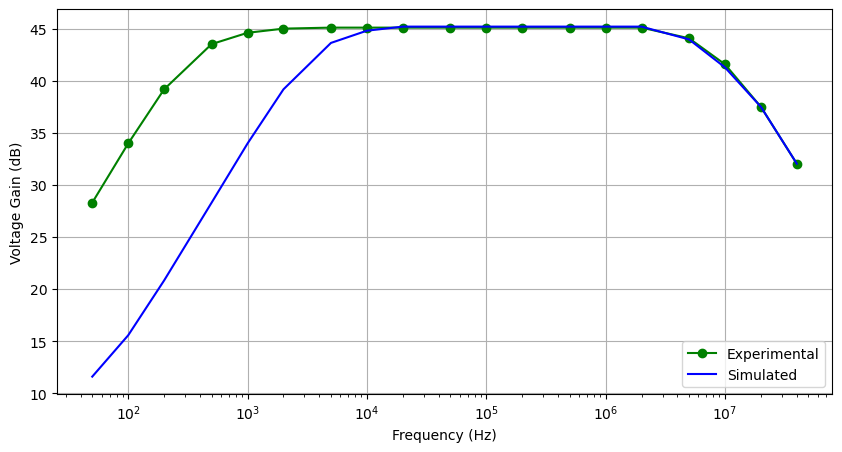
\includegraphics[width=.8\textwidth]{Graph.png}
    \caption{Plot of Frequency Response}
\end{figure}

\section{Discussion}
The experiment focused on analyzing the frequency response of a single-tuned amplifier. The output voltage varied significantly across different frequencies despite a constant input voltage, reflecting typical amplifier behavior. Notably, the experimental and simulated gain values showed discrepancies, likely due to real-world factors like parasitic elements and component tolerances. However, both sets of data exhibited similar overall frequency response curves, indicating a strong correlation between experimental and simulated results. This correlation validates the experimental approach and confirms the theoretical predictions of frequency response for single-tuned amplifiers. The experiment thus successfully demonstrated the amplifier's performance characteristics across a wide frequency range.

\end{document}
